\section{Microprocessor without Interlocked Pipeline Stages}

MIPS exemplifies the principles of Reduced Instruction Set Computer (RISC) architecture, emphasizing streamlined execution through simple instructions and a condensed basic cycle. 
This design aims to enhance the efficiency of Complex Instruction Set Computer (CISC) CPUs.

As a load-store architecture, MIPS operates such that Arithmetic Logic Unit operands are sourced exclusively from the CPU's general-purpose registers, precluding direct retrieval from memory. 
Dedicated instructions are thus essential for operations between registers and main memory.

MIPS is a pipeline architecture, designed for performance optimization by enabling the concurrent execution of multiple instructions from a sequential execution flow.

Additionally, the Instruction Set Architecture (ISA) of MIPS includes a defined set of operations, instruction formats, supported hardware data types, named storage, addressing modes, and sequencing protocols.
\begin{figure}[H]
    \centering
    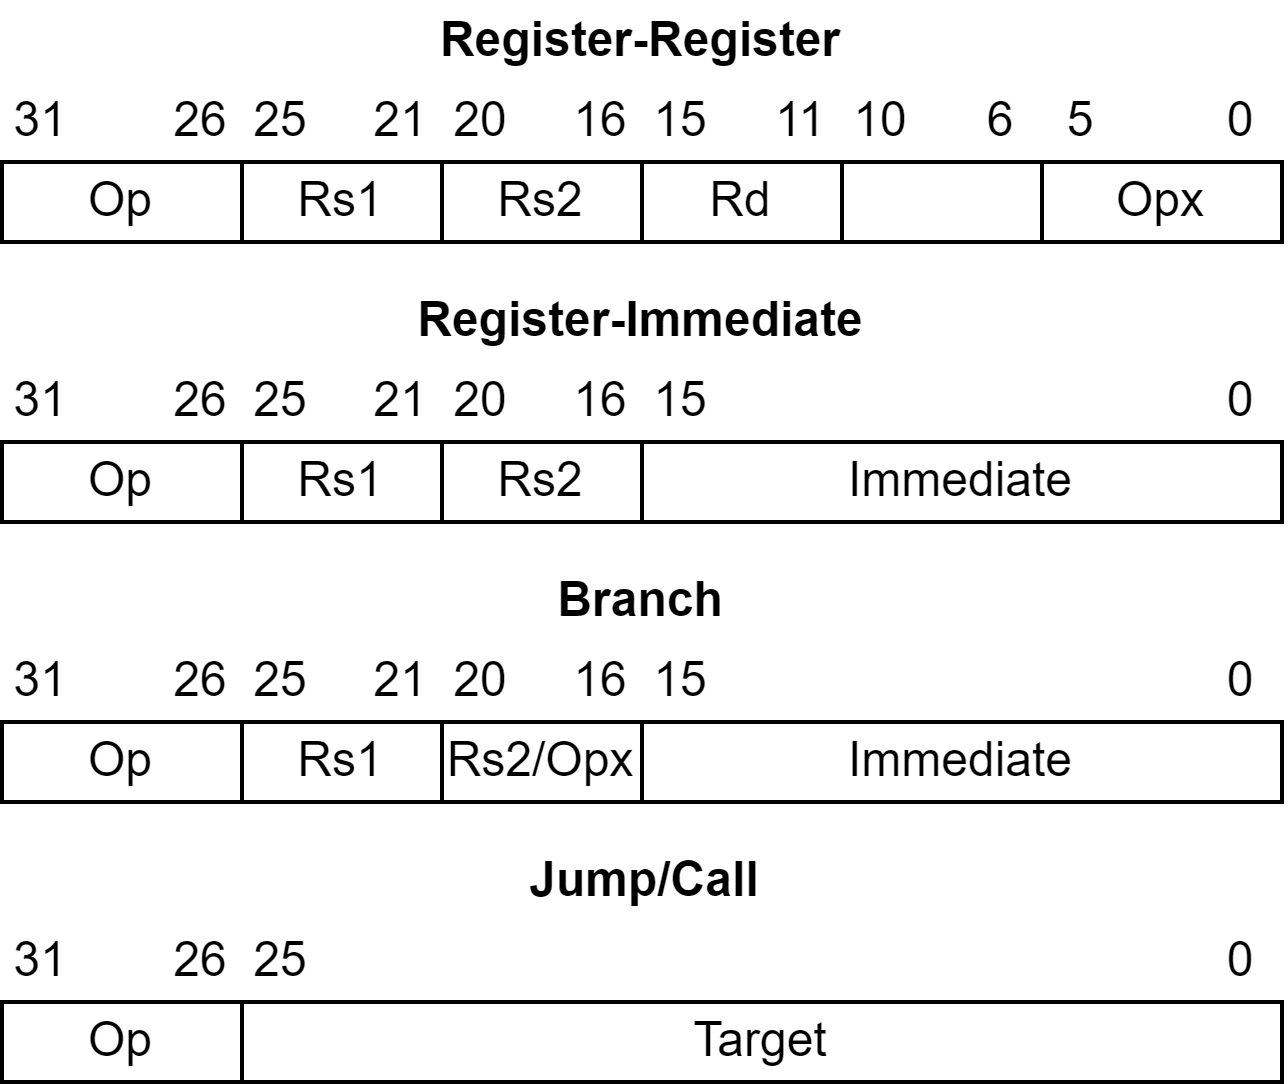
\includegraphics[width=0.4\linewidth]{images/isa.png}
    \caption{MIPS ISA}
\end{figure}

\subsection{MIPS hardware}
Within a MIPS CPU, the data path includes necessary components such as storage, Functional Units (FUs), and interconnects to effectively execute operations. 
In this setup, control points serve as inputs while signals serve as outputs.

The controller, functioning as a state machine, coordinates activities within the data path by directing operations based on the desired function and the signals received.
\begin{figure}[H]
    \centering
    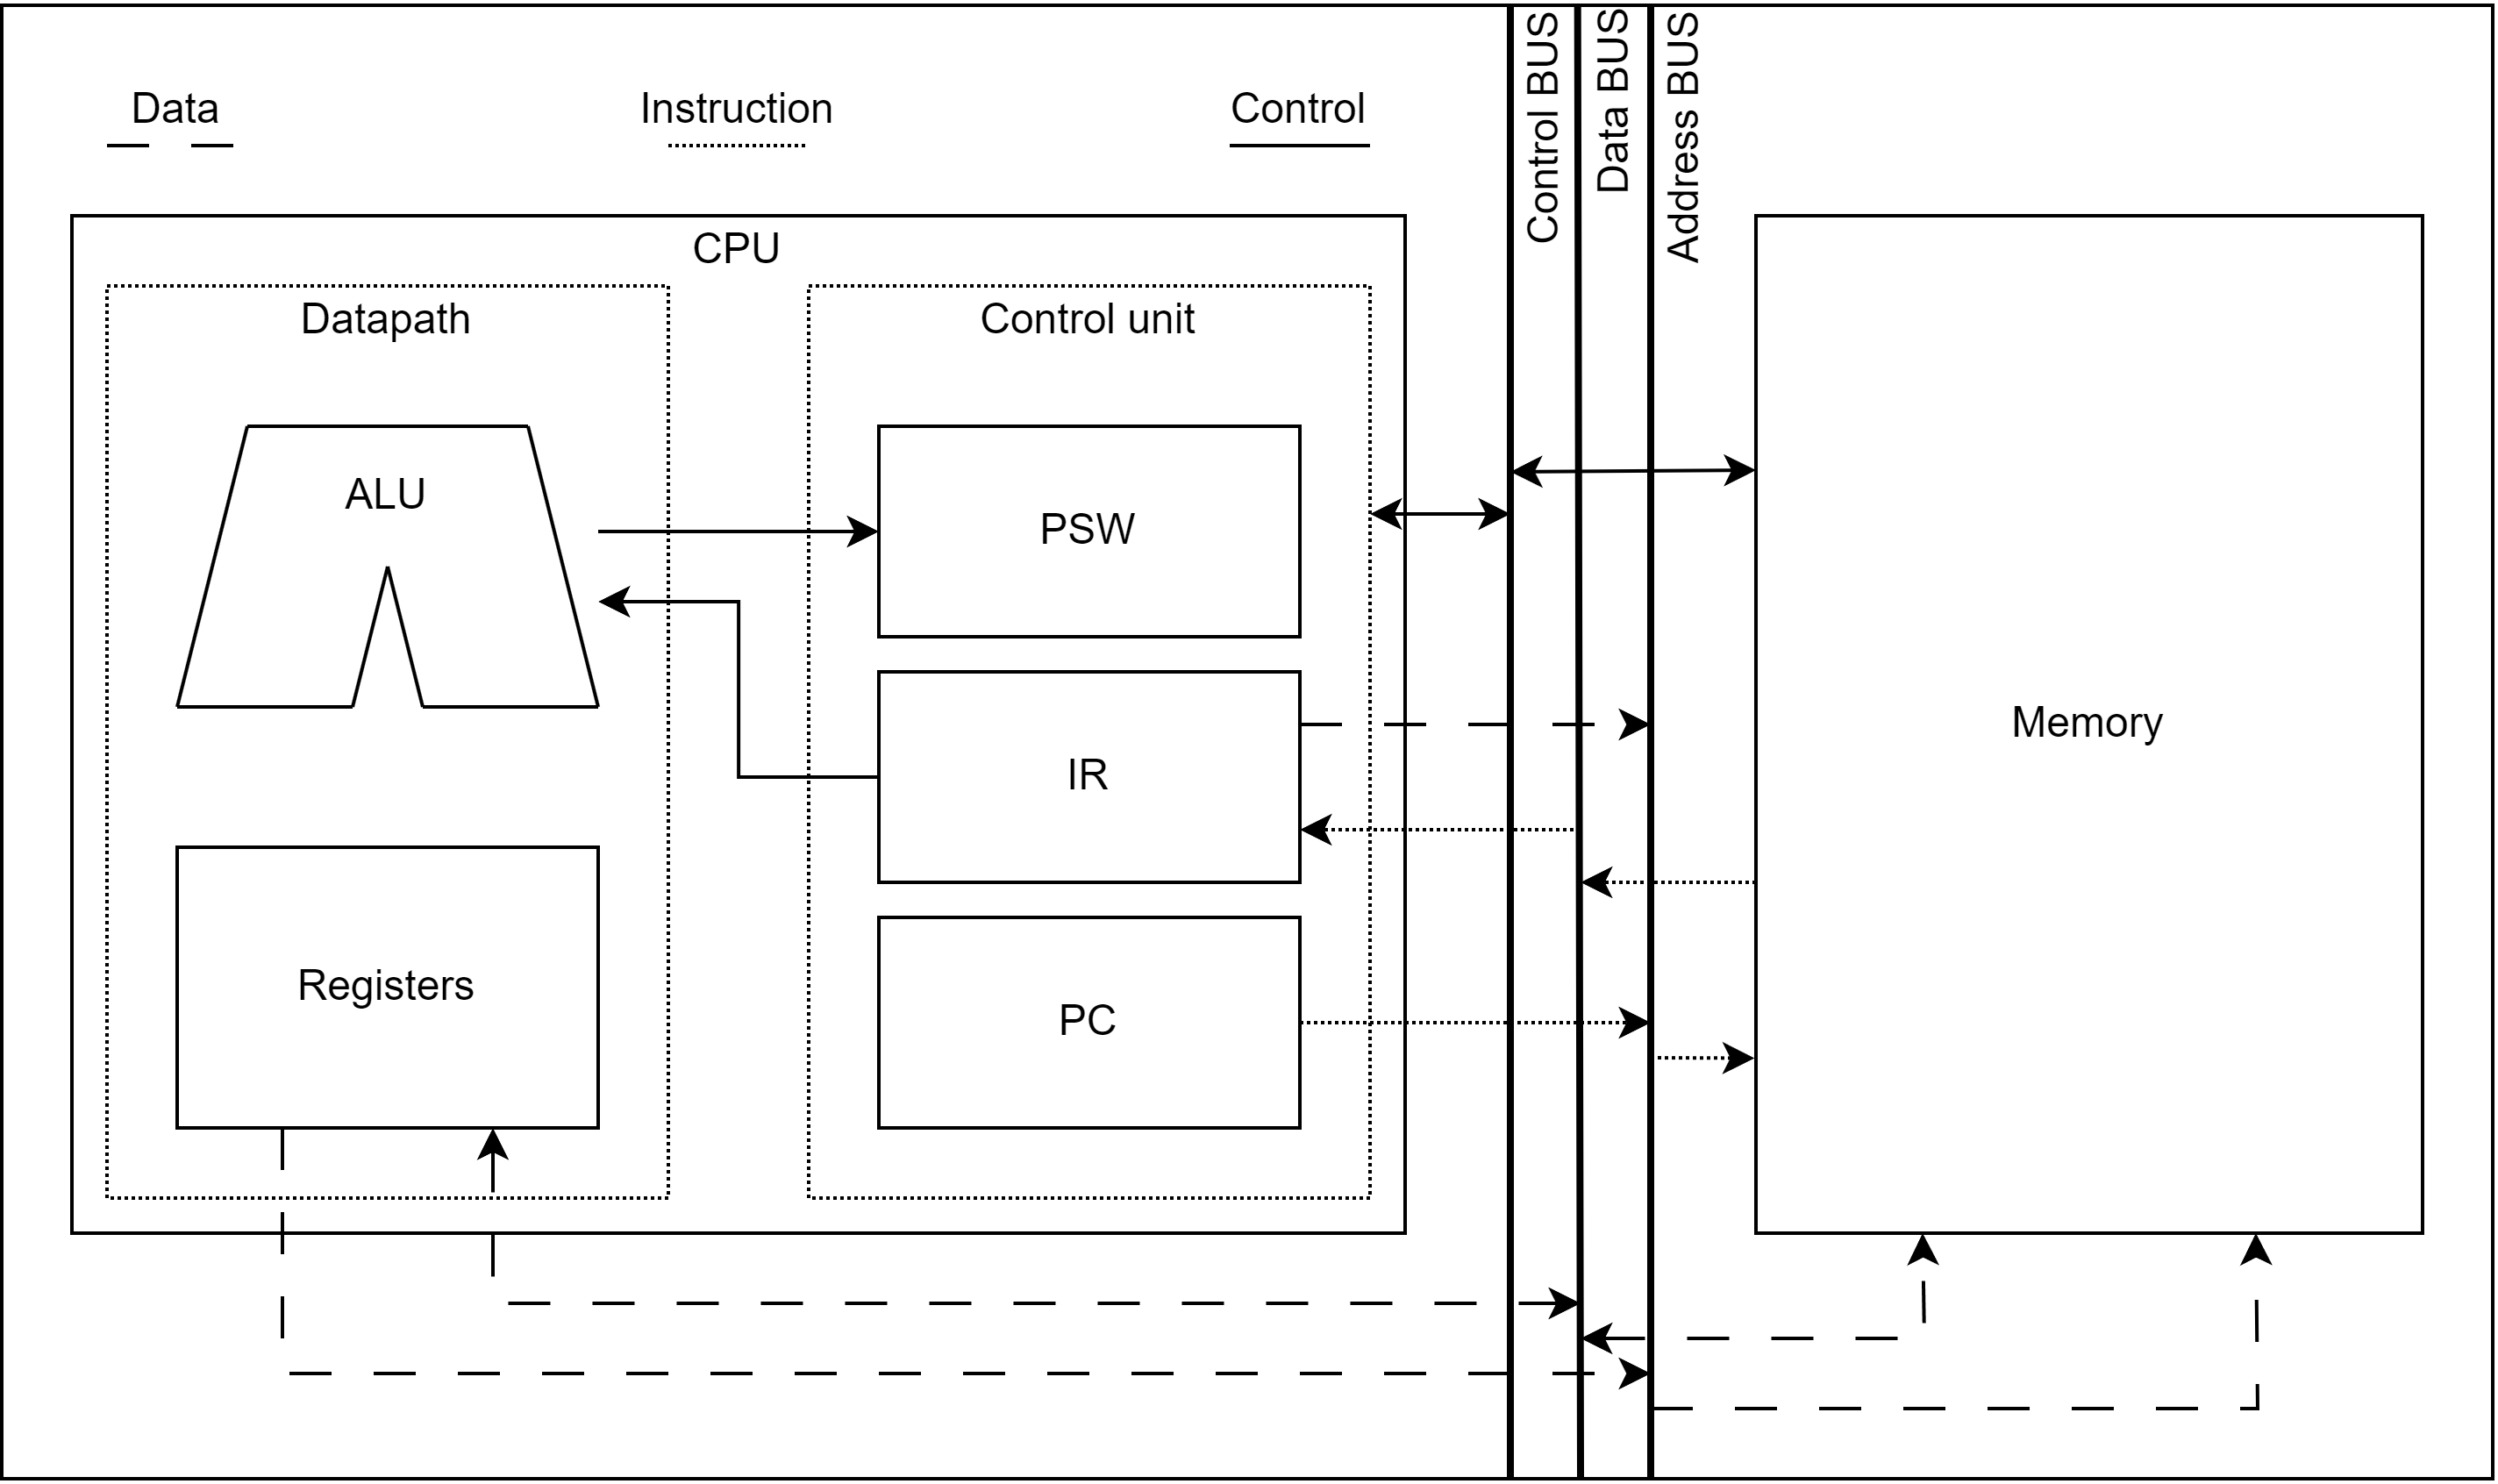
\includegraphics[width=0.75\linewidth]{images/cpu.png}
    \caption{MIPS CPU}
\end{figure}
At the core, a program is segmented into instructions, with the hardware focusing on individual instructions rather than the entire program. 
At a lower level, the hardware divides instructions into clock cycles, with state machines transitioning states with each cycle.

\subsection{MIPS workflow}
Each instruction within the MIPS subset can be executed within a maximum of five clock cycles, as outlined below:
\begin{enumerate}
    \item \textit{Instruction Fetch cycle} (IF): The content of the Program Counter (PC) is transferred into the instruction memory, and the instruction to be executed is retrieved. 
        Then, the PC is incremented by four to point to the next instruction.
    \item \textit{Instruction Decode cycle} (ID): the executing instruction is decoded, and the necessary registers are loaded. 
        If needed, a sign extension of the offset field is performed.
    \item \textit{Execution cycle} (EX): arithmetic operations are performed between registers or between a register and an immediate value. 
        If dealing with a branch or a memory instruction, the address with the offset is computed in this stage. 
        For branches, the registers are compared to determine if the branch is taken or not.
    \item \textit{Memory access cycle} (MEM): for load operations, the value in memory is stored into a register, while for store operations, the register value is saved into main memory. 
        If executing a branch, the value of the PC is updated to the branch address.
    \item \textit{Write Back cycle} (WB): the memory value is saved into the register, finalizing the load operation, and the result of arithmetic operations is saved into the register.
\end{enumerate}
\begin{figure}[H]
    \centering
    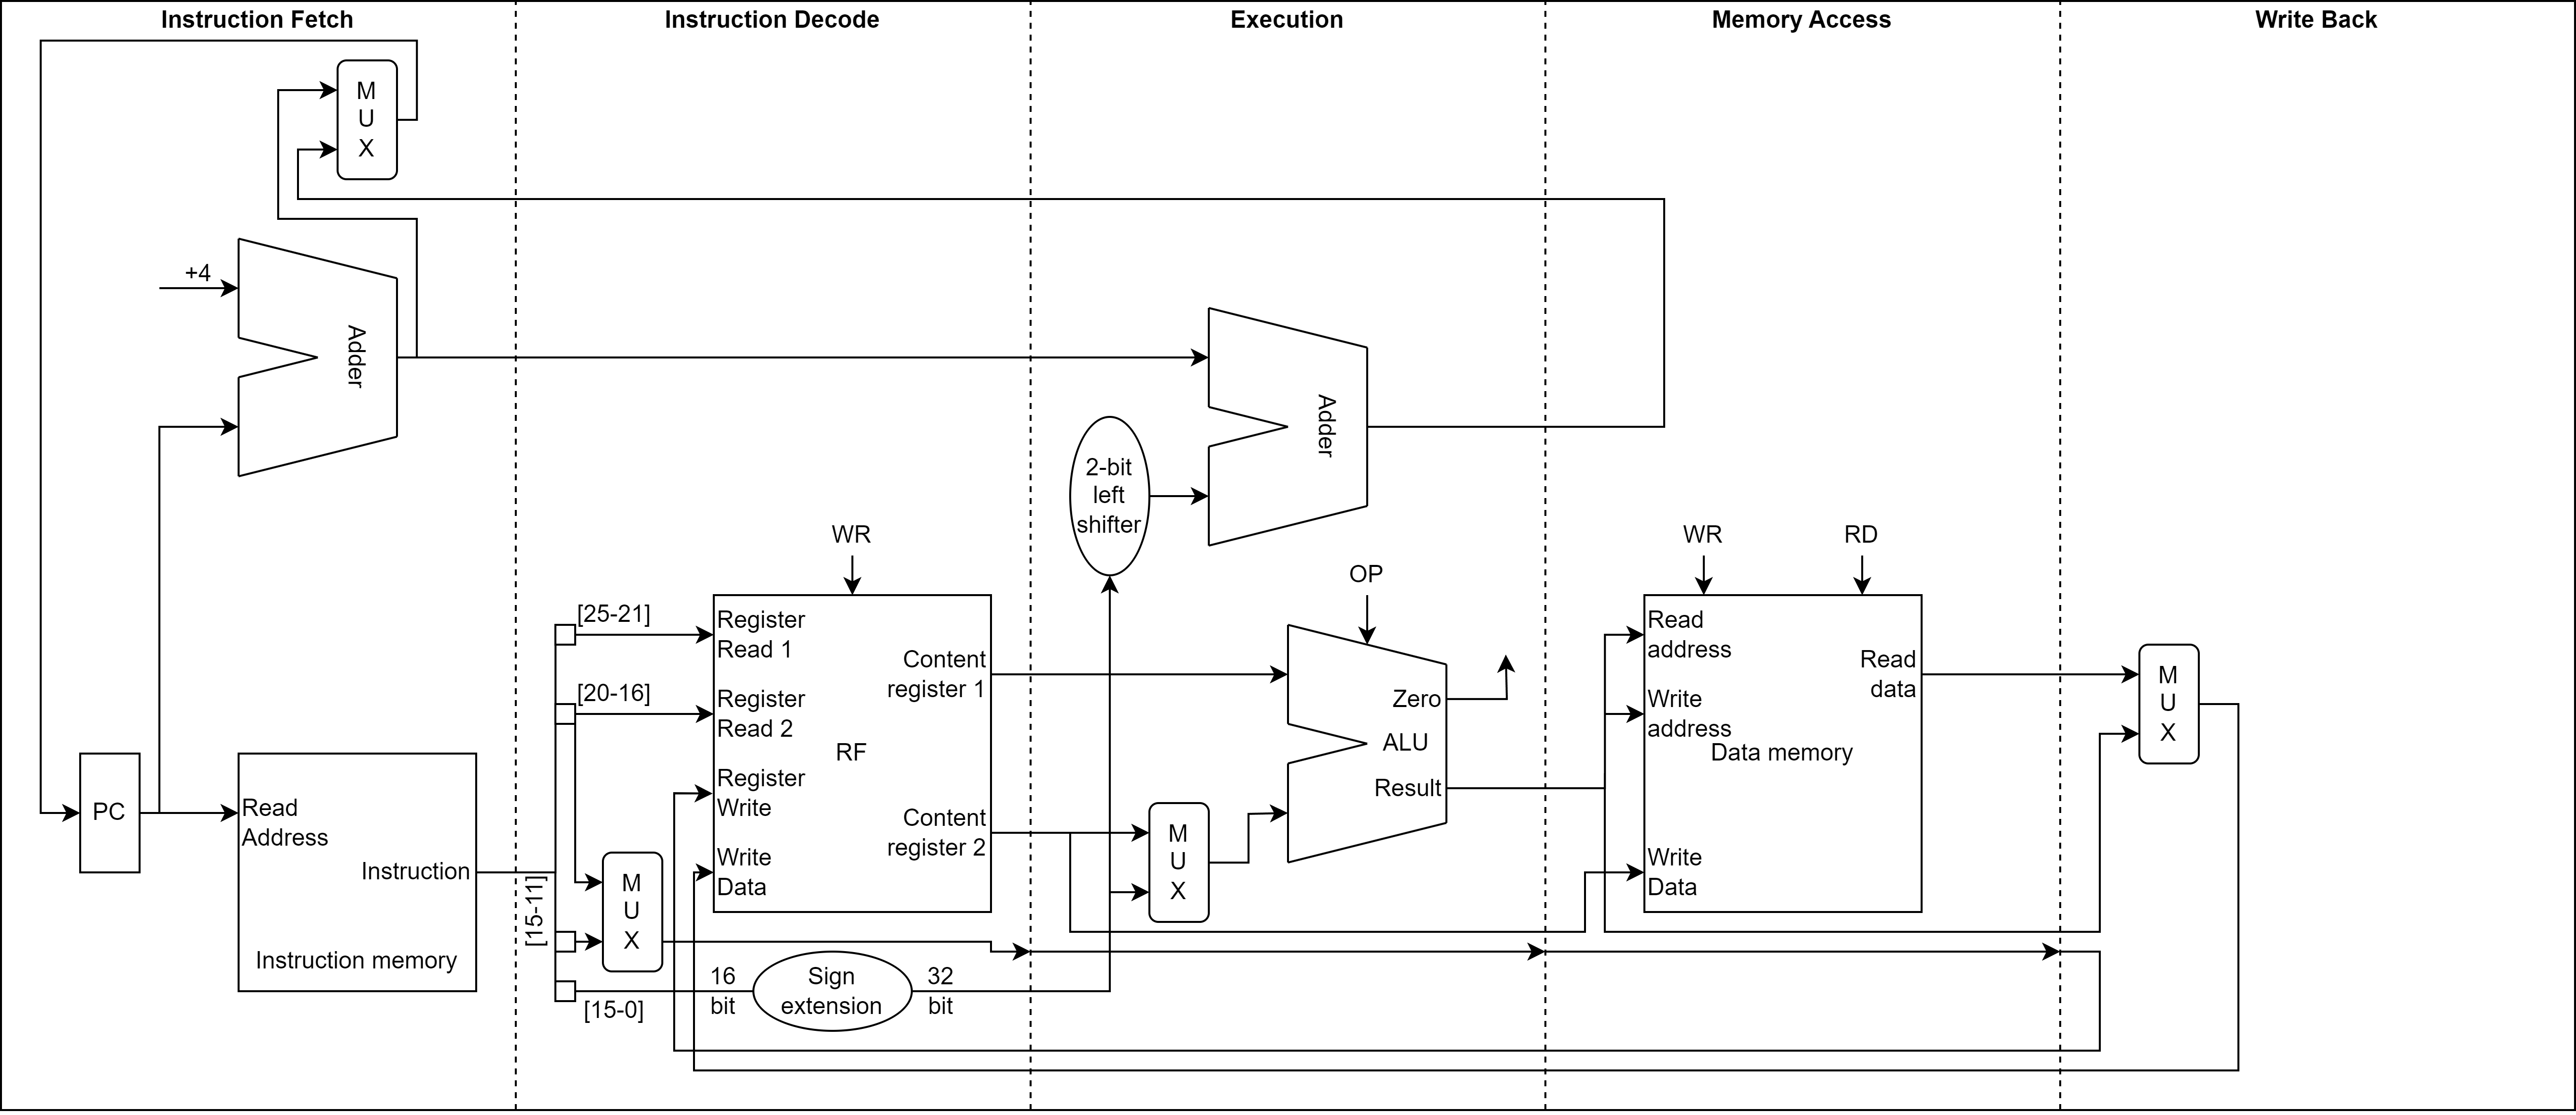
\includegraphics[width=1\linewidth]{images/mips.png}
    \caption{MIPS architecture}
\end{figure}

The duration of each clock cycle is determined by the critical path established by the load instruction, that is of $8$ ns.
We assume a single-clock cycle execution for each instruction, wherein each module is utilized once within a cycle. 
Modules utilized more than once within a cycle necessitate duplication for efficiency. 
Furthermore, to ensure separate functionality, an instruction memory distinct from the data memory is required.

Certain modules must be duplicated, while others are shared across different instruction flows.
To facilitate sharing a module between two distinct instructions, a multiplexer is utilized.

In the multi-cycle implementation of CPU, the execution of instructions spans across multiple cycles, with MIPS typically utilizing five cycles. 
Key aspects of the multi-cycle CPU implementation include: each phase of instruction execution necessitates a clock cycle, modules can be utilized multiple times per instruction across different clock cycles, allowing for potential module sharing, and Internal registers are required to retain values for subsequent clock cycles. 
These registers store data to be utilized in future stages of the instruction execution process.

\subsection{MIPS pipelining}
Pipelining is an optimization method aimed at enhancing performance by overlapping the execution of multiple instructions originating from a sequential execution flow. 
It capitalizes on the inherent parallelism among instructions within a sequential instruction stream.

The fundamental concept involves breaking down the execution of an instruction into distinct phases, also known as pipeline stages. 
Each stage requires only a portion of the time needed to complete the instruction.
These stages are interconnected to form a pipeline, leading to improved efficiency and throughput.
\begin{figure}[H]
    \centering
    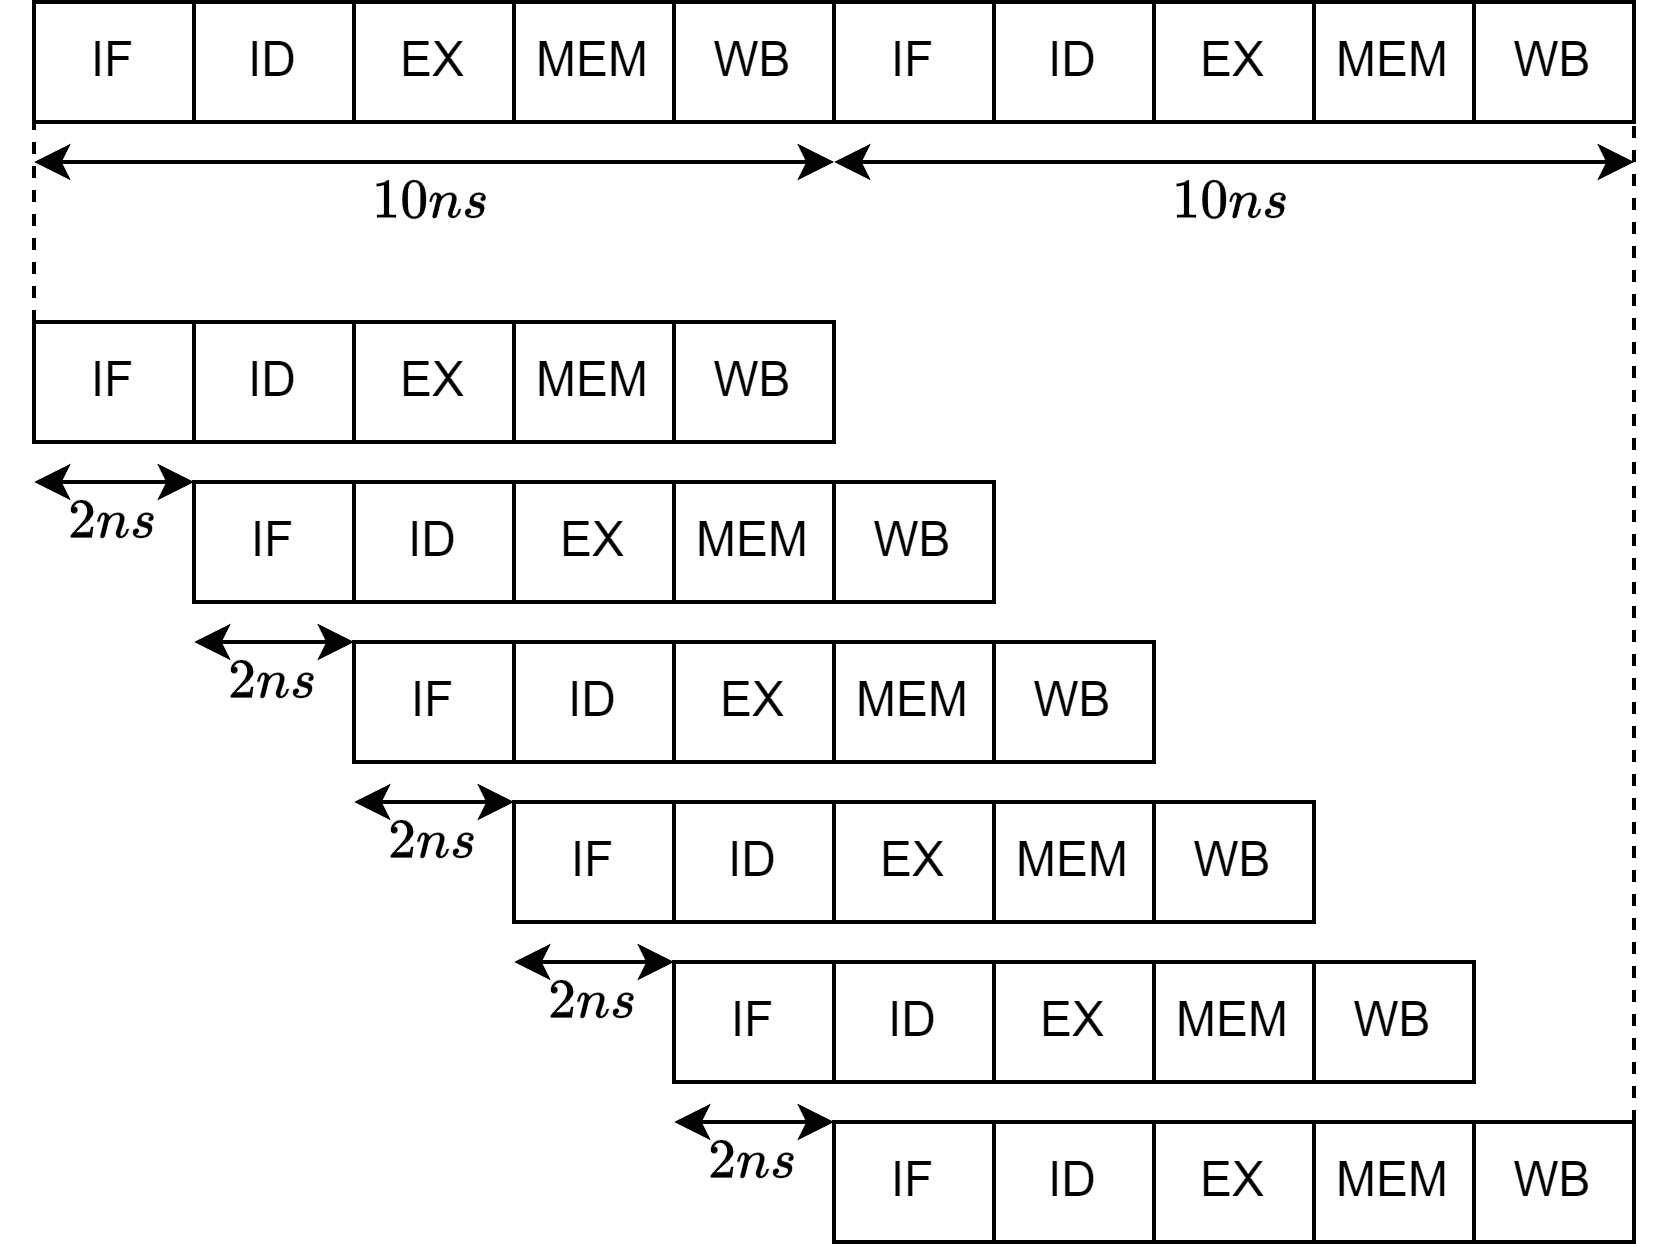
\includegraphics[width=0.5\linewidth]{images/exe.png}
    \caption{Sequential execution and pipelining execution}
\end{figure}

In pipelining, each stage of the pipeline corresponds to the time required to advance an instruction by one clock cycle. 
It's crucial to synchronize the pipeline stages, with the duration of a clock cycle determined by the slowest stage of the pipeline.

The objective is to achieve a balance in the length of each pipeline stage. 
When stages are perfectly balanced, the ideal speedup resulting from pipelining is equal to the number of pipeline stages. 
This ensures optimal utilization of the pipeline, enhancing overall performance and efficiency.

\subsection{Hazards}
A potential concern arises due to the two-stage nature of the Register File: read access during the instruction decode stage and write access during the WB stage. 
When a read and a write operation target the same register within the same clock cycle, it necessitates the insertion of a stall to prevent issues.
\begin{definition}[\textit{Optimized pipeline}]
    An optimized pipeline is achieved when the Register File read operation takes place in the second half of the clock cycle, while the Register File write operation occurs in the first half of the clock cycle.
\end{definition}
Another potential issue is the occurrence of hazards within the pipeline.
Hazards arise when there is a dependency between instructions, and the pipelining process causes a change in the order of accessing operands involved in the dependency, thereby preventing the next instruction from executing during its designated clock cycle.
Hazards diminish the performance from the ideal speedup achieved by pipelining. 
Hazards can be categorized into three main types:
\begin{itemize}
    \item \textit{Structural hazards}: these occur when different instructions attempt to use the same resource simultaneously.
        For example, there may be a conflict when both instructions require access to a single Memory Unit for instructions and data.
    \item \textit{Data hazards}: these occur when an instruction tries to use a result before it is ready. 
    For instance, an instruction might depend on the result of a previous instruction that is still in the pipeline.
    \item \textit{Control hazards}: these occur when a decision regarding the next instruction to execute is made before the condition for the decision is evaluated. 
        For instance, issues arise during conditional branch execution.
\end{itemize}

\subsection{Data hazards}
\paragraph*{Read After Write}
Read After Write (RAW) hazard occurs when an instruction $j$ attempts to read an operand before instruction $i$ has written to it. 
Potential solutions for mitigating this hazard include:
\begin{itemize}
    \item \textit{Compilation techniques}: using no-operation instructions (nop) or instruction scheduling to rearrange instructions so that dependent instructions are not placed too closely together. 
        If all instructions are dependent, inserting nops may be necessary.
    \item \textit{Hardware techniques}: Inserting stalls in the pipeline or utilizing data forwarding. 
        Data forwarding involves using temporary results stored in pipeline registers instead of waiting for results to be written back to the Register File. 
        This technique can often resolve conflicts without introducing stalls. 
        However, for load and use hazards, a stall may still be required to properly resolve the issue.
\end{itemize}

\paragraph*{Write After Write}
Write After Write (WAW) hazard arises when instruction $j$ writes operand before instruction $i$ writes to it.
This situation can lead to incorrect order of write operations. 
Notably, this type of hazard does not occur in the MIPS pipeline since all register write operations occur in the WB stage.

\paragraph*{Write After Read}
Write After Read (WAR) hazard arises when an instruction $j$ writes operand before instruction $i$ reads from it.
However, such hazards do not occur in the MIPS pipeline because operand read operations occur in the instruction decode stage, while write operations occur in the WB stage.